\documentclass[11pt,a4paper]{article}
\usepackage{fontspec}
\setmainfont{TeX Gyre Pagella}
\newfontfamily\headfont{Inter}[UprightFont=*-ExtraBold,BoldFont=*-ExtraBold,Extension=.otf,Path=/usr/share/fonts/opentype/inter/]
\usepackage[a4paper,margin=2.3cm]{geometry}
\usepackage{graphicx,booktabs,float,caption,array,xcolor,longtable}
\usepackage{xurl}
\usepackage[hidelinks]{hyperref}
\usepackage{titlesec}
\usepackage[round]{natbib}
\usepackage{setspace}
\setstretch{1.05}
\renewcommand{\topfraction}{0.9}
\renewcommand{\bottomfraction}{0.8}
\renewcommand{\textfraction}{0.1}
\renewcommand{\floatpagefraction}{0.75}
\setlength{\parindent}{0pt}
\setlength{\parskip}{0.55em}
\titleformat{\section}{\headfont\Large}{\thesection}{0.8em}{}
\titleformat{\subsection}{\headfont\large}{\thesubsection}{0.8em}{}
\captionsetup{font=small,labelfont=bf}
\urlstyle{same}
\hypersetup{pdftitle={Every Embassy in the World},pdfauthor={Tristan Hotham}}

\begin{document}
\begin{center}
{\Large\bfseries Every Embassy in the World\par}
\vspace{0.4em}
{\large The world's diplomatic missions from open data,\\and the diplomatic web from the Amarna letters to today\par}
\vspace{1.2em}
{\large Tristan Hotham\par}
\vspace{0.3em}
{\small Independent researcher\\
ORCID: 0000-0003-4931-9349\\
DOI: https://doi.org/10.5281/zenodo.23899269\par}
\vspace{0.8em}
2026
\end{center}

\begin{quote}
\small
\begin{center}\textbf{Abstract}\end{center}
I build an open gazetteer of the world's current diplomatic missions by cleaning, merging and checking 17,573 OpenStreetMap objects tagged as diplomatic and the embassy, consulate and representative-office items of Wikidata. The result holds 15,584 located missions sent by 198 states, the European Union and the Sovereign Order of Malta, in 1,031 cities, plus 1,191 missions known only as country pairs. 9,822 ordered pairs of states, 25.2\% of those possible, have an embassy-level mission. Totals of posts agree with the Lowy Institute Global Diplomacy Index to within 85\% to 105\% for the seven countries it reports in its key findings. China has the widest embassy-level network (178 states) and United States the most posts (279); Washington, D.C. hosts the most embassies (181) and Barcelona the most consulates (83). I document capitals whose embassies stayed behind or moved, special cases of contested recognition as the data record them, and per-country coverage against the Correlates of War Diplomatic Exchange data, which I also use to trace the diplomatic web from 23 states and 198 links in 1817 to 192 states and 8,110 links in 2005, with ambassador-level links rising from 11.6\% to 92.7\%. A small sample of 52 famous missions from 2400 BC to 1815 sets the modern network in a longer history; 42 of its 60 dated lines are confirmed in the cited articles.

\textbf{Keywords:} diplomacy; embassies; consulates; OpenStreetMap; Wikidata; Correlates of War; diplomatic networks; open data
\end{quote}

\section{Introduction}
Embassies are the most visible infrastructure of international relations: buildings in foreign capitals that signal recognition, interest and the willingness to pay for a permanent presence. Diplomatic representation has long been used as a measure of status and of the structure of the state system \citep{bayer}, and the Lowy Institute's Global Diplomacy Index counts the networks of 66 countries in detail \citep{lowy}. What has been missing is an open, global, located map of every mission, which open collaborative data now make possible.

This paper builds such a map, checks it against independent counts, and uses it to describe the present network: who is present where, where embassies cluster, which capitals they have not followed, and how the data record cases where recognition is contested. It then sets the present against the Correlates of War record of 1817 to 2005, and against a small sample of earlier missions. The interactive version lets readers draw any country's network and see who is present in any capital (\url{https://maps.tristanhotham.com/embassies/}).

\section{Data}
\textbf{OpenStreetMap.} I start from 17,573 objects tagged office=diplomatic or amenity=embassy, fetched through the Overpass API in 2026 \citep{osm}. Tags give the kind of mission (diplomatic=embassy, consulate or liaison, refined by embassy=high\_commission, nunciature, delegation, mission, residence or branch\_embassy and consulate=consulate\_general, honorary\_consul and others), the sending state (country, an ISO 3166 code) and the receiving state or organisation (target). 6,802 of the kept objects link to a Wikidata item.

\textbf{Wikidata.} The Wikidata extract \citep{wikidata} requested items of six classes. Checking the items of each class by name showed two to be the wrong classes: one holds 20,523 schools and colleges and another 5,556 television channels; fewer than 1\% of their items are named as missions, against 97.2\% of the embassy class. They were dropped. The embassy (8,529 items), consulate (350) and representative office (152) classes were kept. Items give the operator (sending state), country, coordinates for some, and inception and end dates.

\textbf{Correlates of War.} The Diplomatic Exchange data set v2006.1 \citep{bayer} records, for every pair of states in the system and about every five years from 1817 to 2005 (38 waves), the level at which each is represented in the other: none, charg\'e d'affaires, minister, ambassador or other. Every pair appears in both orders and the codings agree. In the 1950 to 1965 waves every represented pair is coded ``other'': levels were not recorded, so I count representation for those years but not ambassadors.

\textbf{Benchmarks and geography.} The Lowy Institute's 2024 key findings give total posts for seven countries \citep{lowy}. Natural Earth supplies borders and populated places \citep{naturalearth}.

\section{Methods}
\textbf{Classification and cleaning.} Each OpenStreetMap object is given one of eleven types: embassy, high commission, apostolic nunciature, delegation, interests section, permanent mission to an organisation, consulate-general, consulate, honorary consulate, representative or liaison office, and embassy section or office (trade, cultural and consular sections). The first five are ``embassy level''. Names in English and 22 other languages are matched with regular expressions to refine types where tags are missing. I dropped 775 residences, 84 offices of international organisations, 289 objects whose sending state could not be determined and 564 that were not diplomatic.

\textbf{Sending and receiving states.} The sending state comes from the country tag, else the linked Wikidata item, else the name, matched against country names and demonyms in many languages with longer names matched first (so that ``Niger'' does not match inside ``Nigeria''). An explicit English name (``Embassy of Montenegro'') overrides a conflicting tag. A bare ``Republic of China'' is treated as ambiguous. 465 missions take their sender from a name. Missions tagged with sub-national senders (German L\"ander, Spanish and Italian regions, Qu\'ebec, Hong Kong) are kept but separated (129). The receiving state is the territory in which the mission stands (Natural Earth 1:10m), except embassies to the Holy See, which stand in Rome, and permanent missions, which are accredited to an organisation. Every mission is named after the nearest large city.

\textbf{Merging.} Missions of the same kind from the same sender to the same receiver within 350 m are merged (352); objects sharing a Wikidata identifier are also merged. Wikidata items are then linked through OpenStreetMap's wikidata tags (5,731), matched by sending and receiving state (1,722), added as points when they have coordinates that OpenStreetMap lacks (81), or kept as country pairs without a location (1,191). Items with an end date (244) or of states that no longer exist are dropped.

\textbf{Corrections.} 12 states recognise Taiwan \citep{reuters}. Embassy-level records between Taiwan and other states are either working offices named as embassies, counted as representative offices, or records of embassies closed when recognition switched, which are flagged as out of date and excluded (13 records). 3 hand corrections are listed in the merge log.

\textbf{Coverage.} For each state I compare the number of states in which it has an embassy-level mission in 2026 with the number in which the Correlates of War data record it as represented in 2005, and likewise for missions hosted. A ratio of at least 0.8 is ``good'', 0.5 to 0.8 ``partial'' and below 0.5 ``thin''. The benchmark is crude: many embassies have opened since 2005 and the 2005 data count non-resident accreditation in some cases.

\textbf{Deep history.} The 60 lines before 1817 are a hand-compiled sample of famous missions, letters, treaties, tribute missions, congresses and the first resident embassies, with conventional dates, approximate court locations and an English Wikipedia article as the cited source for each (44 articles). Each date was checked against its cited article: 42 lines are confirmed (the year appears in the article), 10 approximate (the article gives a nearby year) and 8 not confirmed (Table~\ref{tab:deep}).

\section{Results}
\subsection{The map}
The gazetteer holds 15,584 missions (Figure~\ref{fig:map}): 8,917 embassies, 406 high commissions, 92 nunciatures, 148 delegations, 352 permanent missions, 1,857 consulates-general, 1,528 consulates, 1,867 honorary consulates, 239 representative offices and 173 embassy sections. 15,503 come from OpenStreetMap and 81 from Wikidata. Of the 9,822 embassy-level pairs of states, 7,099 are in both sources, 1,604 only in OpenStreetMap and 1,154 only in Wikidata. 4,002 unordered pairs have embassies both ways and 1,818 ordered pairs are one-way.

\begin{figure}[tbp]\centering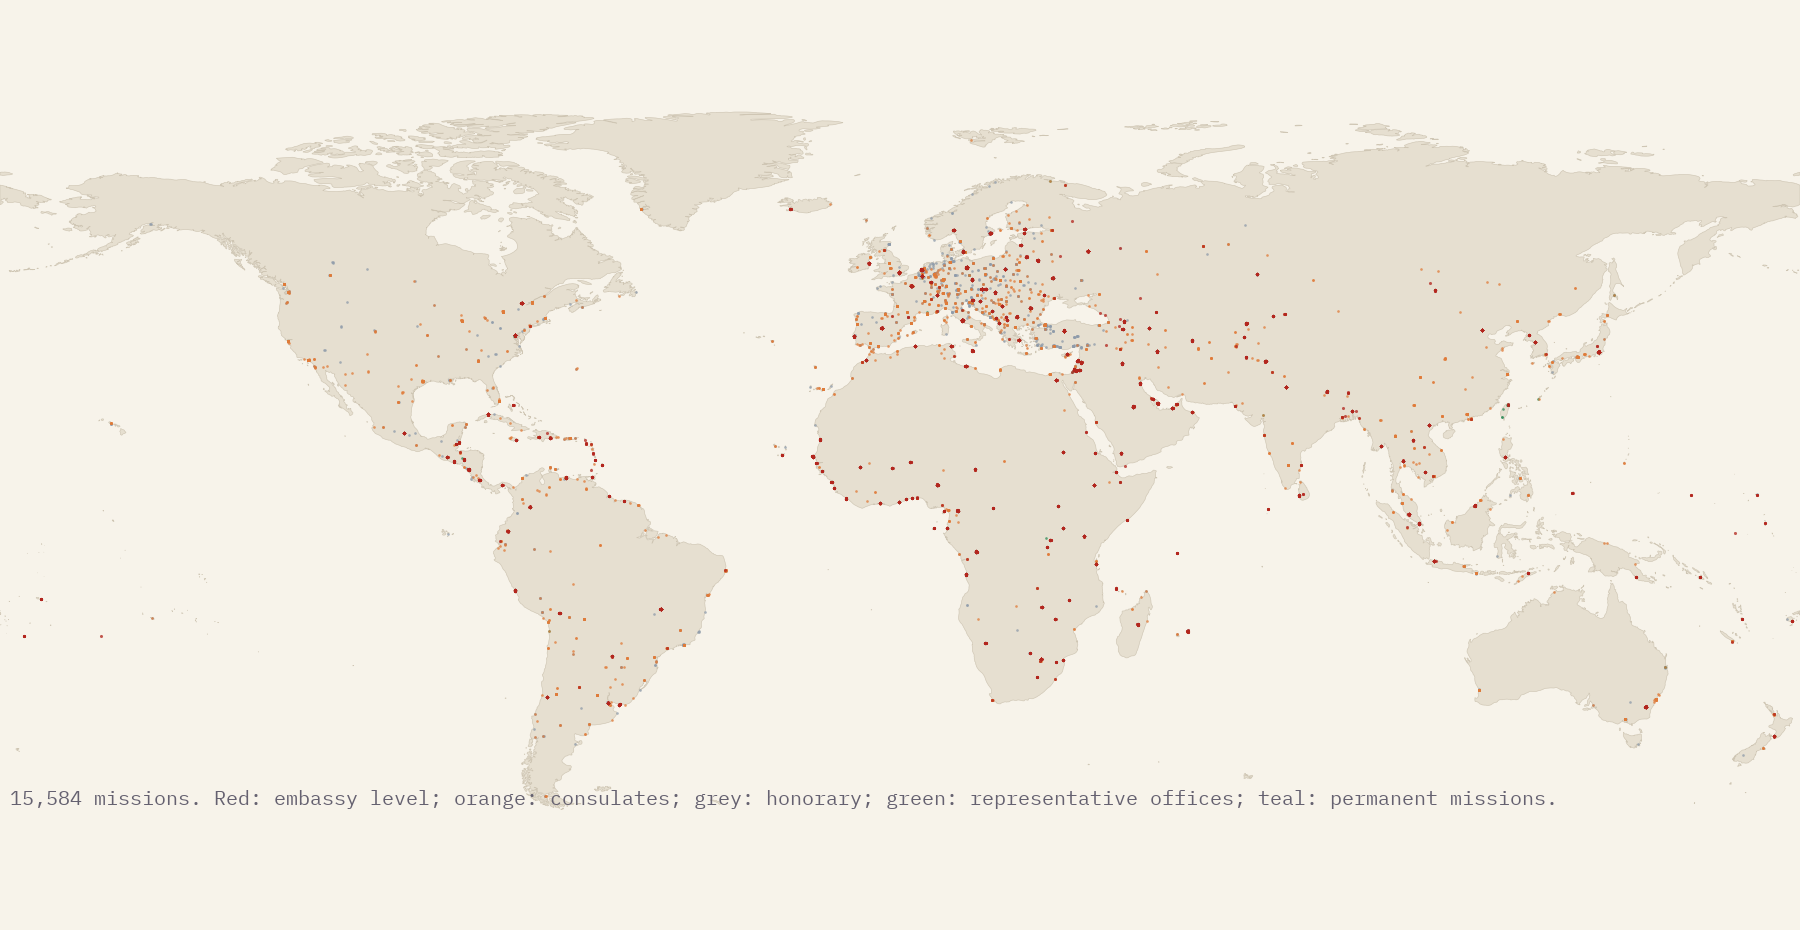
\includegraphics[width=\textwidth]{f_map.png}
\caption{Every mission in the gazetteer, coloured by kind.}\label{fig:map}\end{figure}

\subsection{Networks and the Lowy benchmark}
China has embassy-level missions in 178 states, United States in 168 and France in 166 (Figure~\ref{fig:net}). Counting all posts except honorary consulates, United States has 279 and China 258. Against Lowy's totals the gazetteer finds between 85\% and 105\% (Table~\ref{tab:lowy}). The European Union runs 130 embassy-level delegations and the Holy See 88 nunciatures, the 33rd largest network, for a population of about 825. Figure~\ref{fig:ex} draws four networks.

\begin{table}[tbp]\centering\small\caption{Posts (all missions except honorary consulates, by city) against the Lowy Institute Global Diplomacy Index 2024, and the largest embassy-level networks.}\label{tab:lowy}\begin{tabular}{lrrr@{\hspace{2.2em}}lr}\toprule Country & Lowy & Here & Share & Embassy-level network & States\\\midrule
China & 274 & 258 & 94\% & China & 178\\
United States & 271 & 279 & 103\% & United States & 168\\
Turkiye & 252 & 249 & 99\% & France & 166\\
Japan & 251 & 232 & 92\% & United Kingdom & 160\\
Indonesia & 130 & 133 & 102\% & Japan & 159\\
Australia & 124 & 130 & 105\% & Germany & 155\\
Taiwan & 110 & 93 & 85\% & Turkiye & 148\\
 & & & & Russia & 143\\
 & & & & Brazil & 135\\
 & & & & India & 133\\
\bottomrule\end{tabular}\end{table}

\begin{figure}[tbp]\centering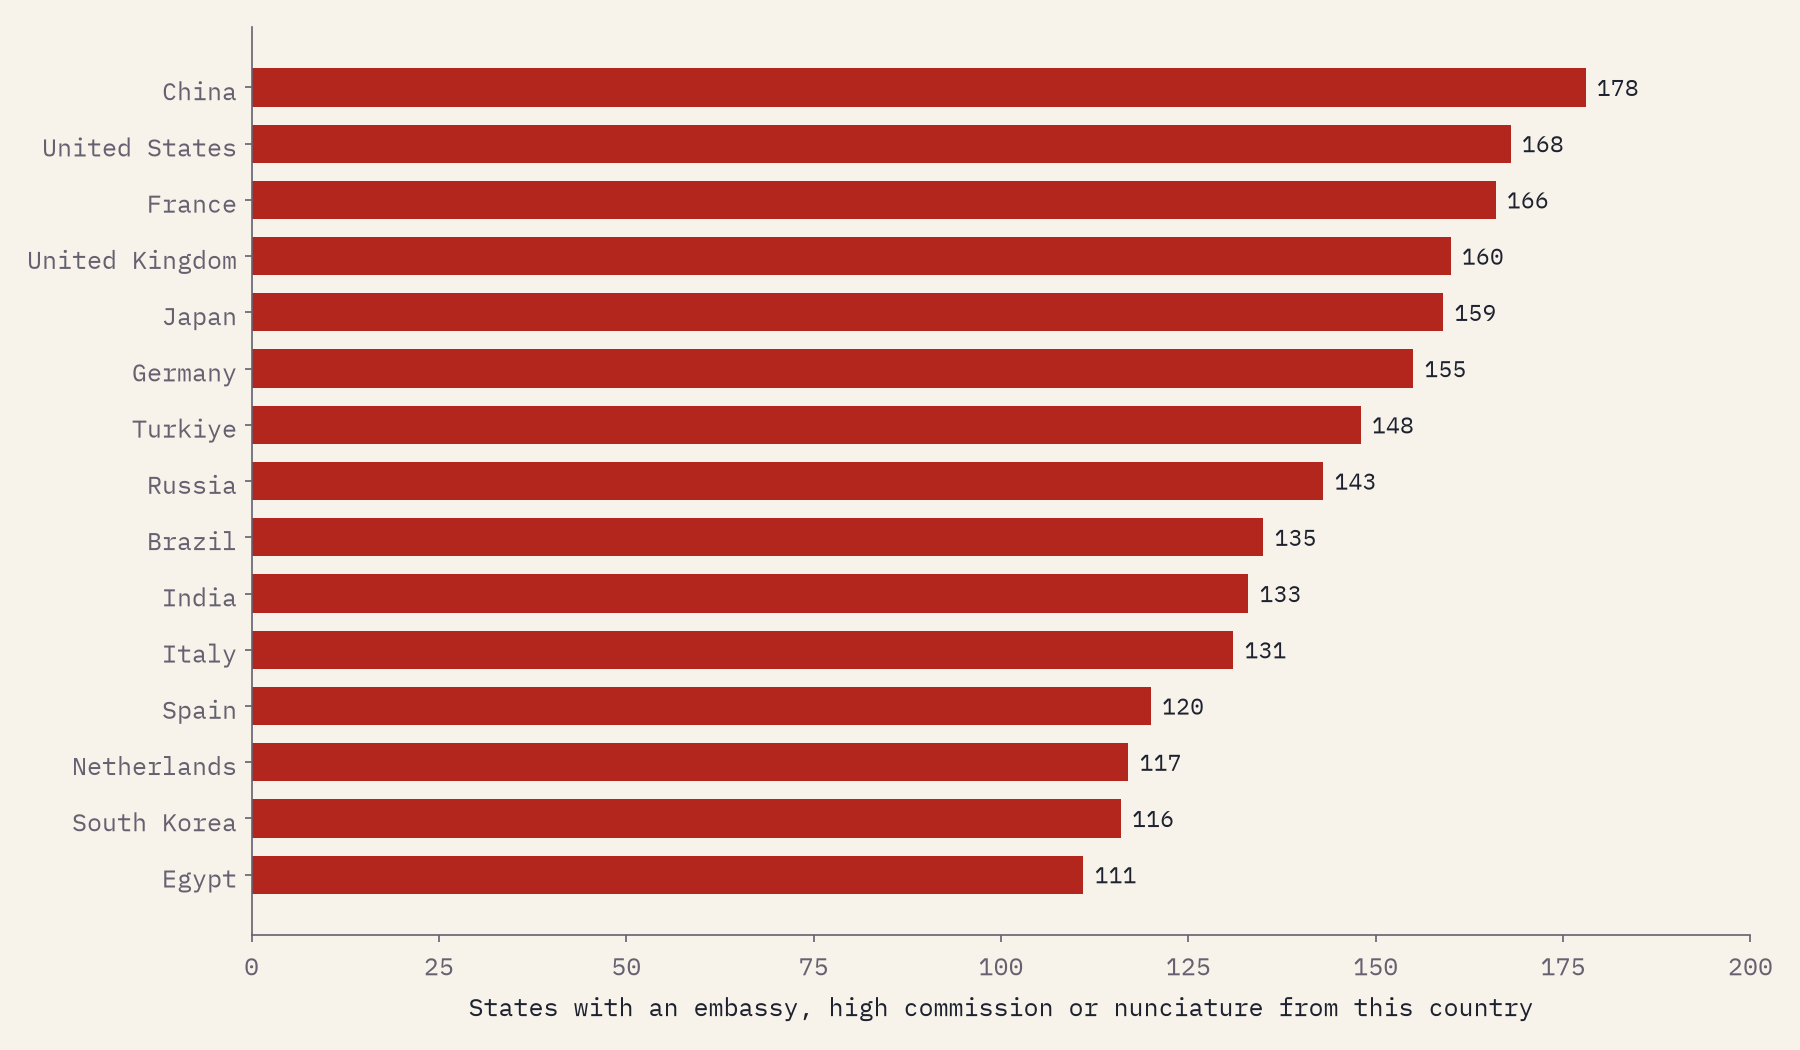
\includegraphics[width=\textwidth]{f_networks.png}
\caption{The largest embassy-level networks: states in which each country has an embassy, high commission or nunciature.}\label{fig:net}\end{figure}

\begin{figure}[tbp]\centering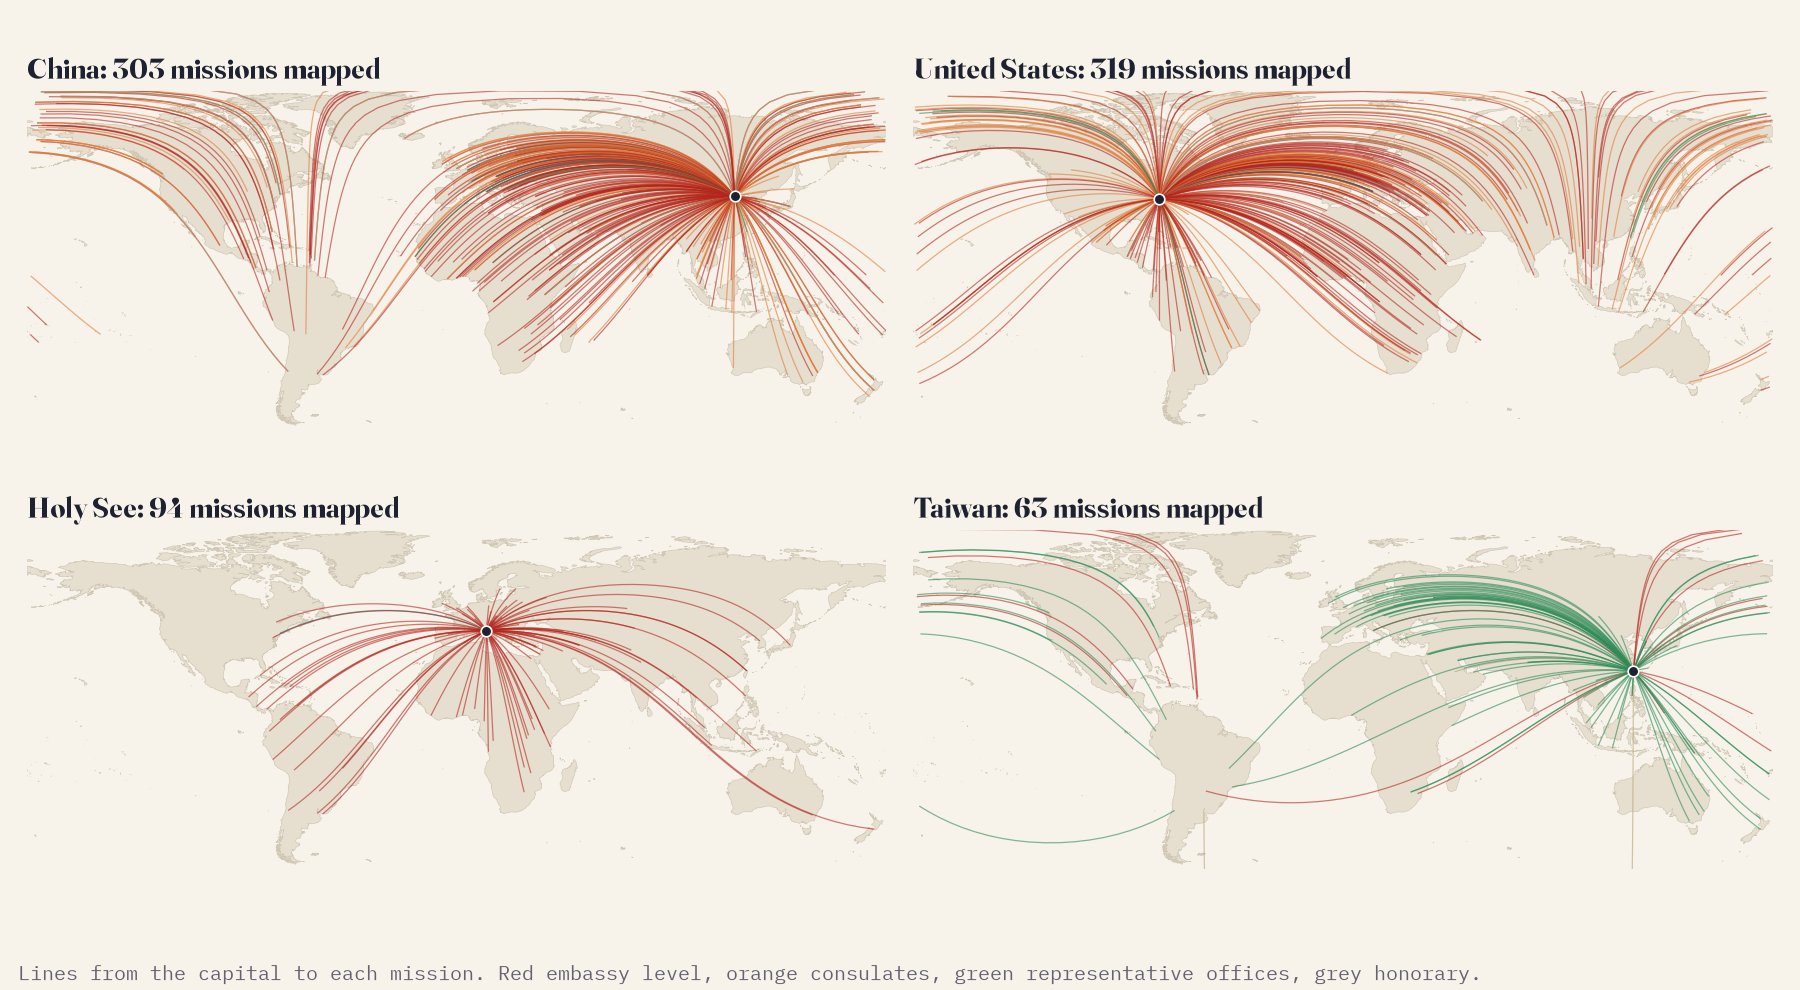
\includegraphics[width=\textwidth]{f_examples.png}
\caption{Four networks, drawn from the capital to every mapped mission (and to the receiving capital for Wikidata pairs without location).}\label{fig:ex}\end{figure}

\subsection{Capitals and clusters}
Washington, D.C. hosts 181 embassies, Brussels 178, Paris and London 170 each (Figure~\ref{fig:cities}). Barcelona has the most career consulates (83), ahead of Istanbul (73). The densest kilometre is around United Nations headquarters in New York (182 missions within 1 km of a point), then Washington (95) and Beijing (73). Liechtenstein hosts no resident embassy.

\begin{figure}[tbp]\centering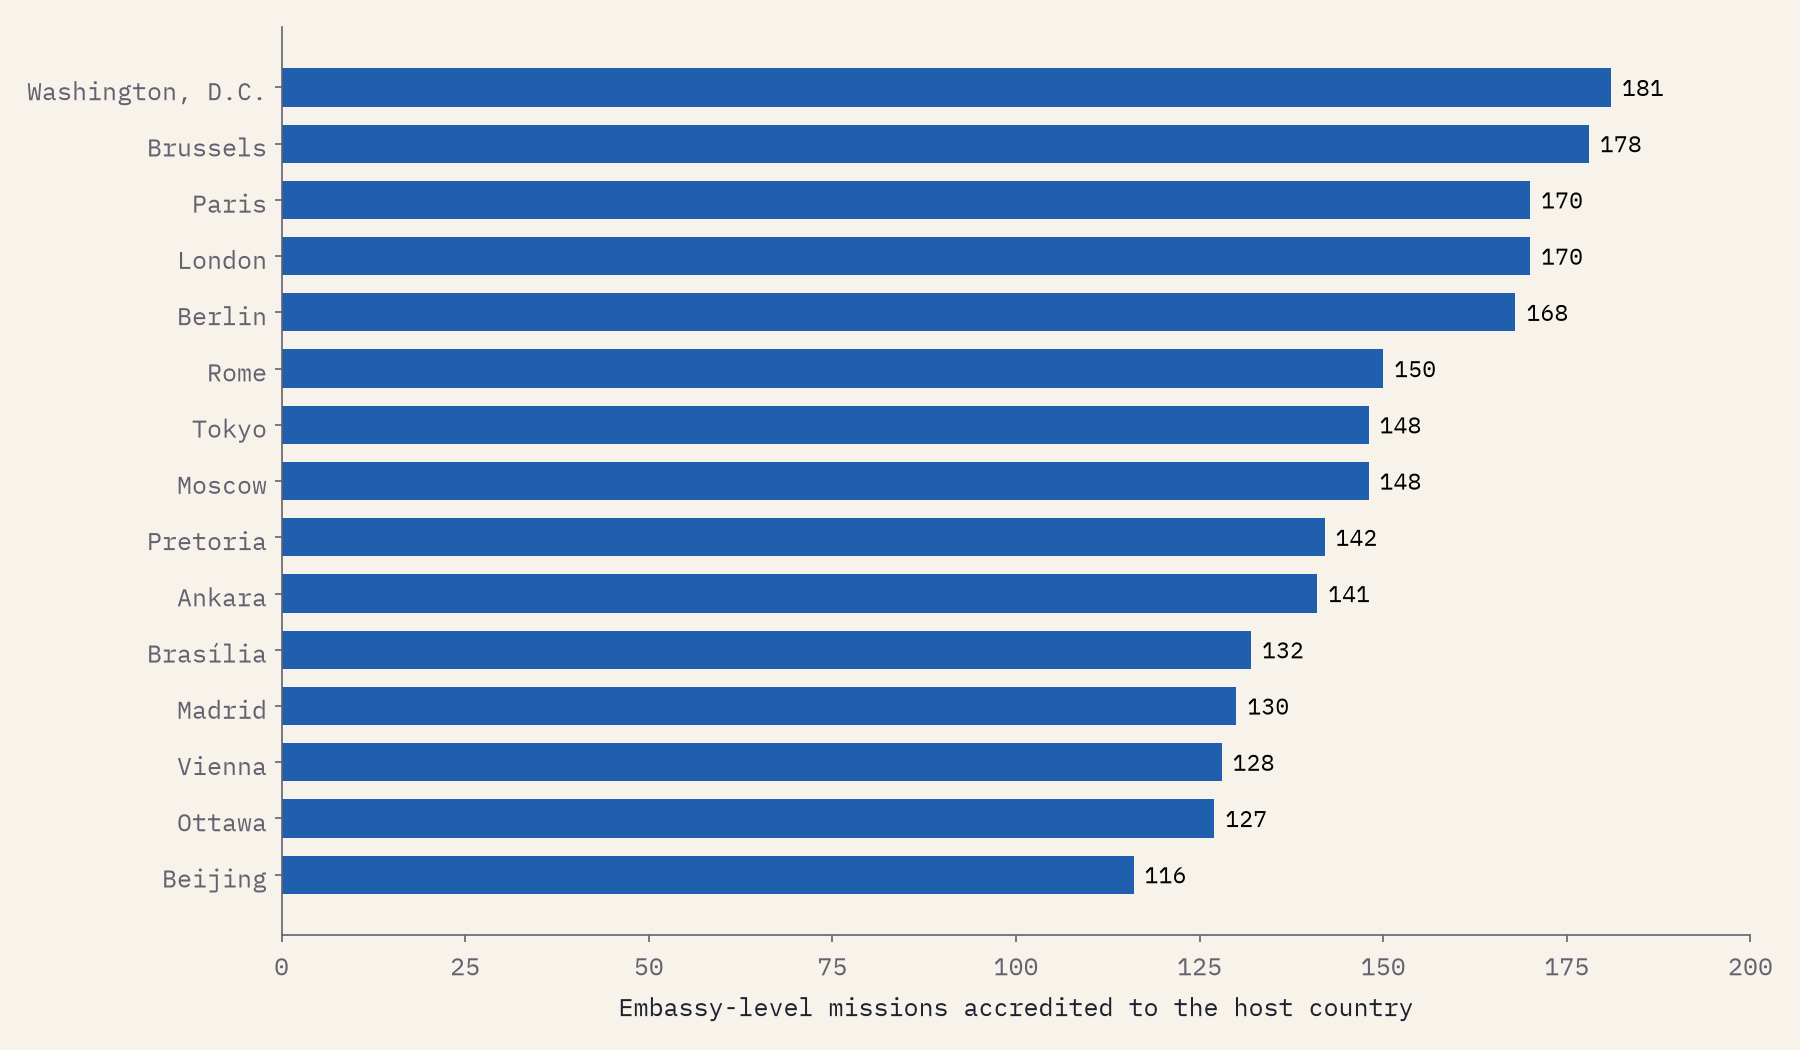
\includegraphics[width=\textwidth]{f_cities.png}
\caption{Cities hosting the most embassy-level missions accredited to their own country.}\label{fig:cities}\end{figure}

\subsection{Capitals the embassies did not follow}
In 10 states the official capital is not where most embassies are (Table~\ref{tab:seats}). Of 82 embassies to Israel, 79 are in the Tel Aviv area and 3 in Jerusalem; the status of Jerusalem is disputed and the data simply record locations. Lagos keeps 24 consulates while 74 embassies are in Abuja; Rio de Janeiro keeps 31 consulates; Bern has 85 embassies and Geneva 58 permanent missions.

\begin{table}[tbp]\centering\small\caption{States whose official capital is not where most embassies to them are (embassy-level missions in each city).}\label{tab:seats}\begin{tabular}{llrlr}\toprule State & Official capital & Embassies & Embassy city & Embassies\\\midrule
Israel & Jerusalem & 3 & Tel Aviv & 79\\
Bolivia & Sucre & 0 & La Paz & 33\\
Cote d'Ivoire & Yamoussoukro & 0 & Abidjan & 42\\
Tanzania & Dodoma & 0 & Dar es Salaam & 61\\
Netherlands & Amsterdam & 0 & The Hague & 111\\
Sri Lanka & Sri Jayawardenepura Kotte & 0 & Colombo & 38\\
Benin & Porto-Novo & 0 & Cotonou & 19\\
Myanmar & Naypyidaw & 0 & Yangon & 46\\
Burundi & Gitega & 0 & Bujumbura & 16\\
Palau & Ngerulmud & 0 & Koror & 4\\
\bottomrule\end{tabular}\end{table}

\subsection{Contested cases, as recorded}
The data record Taiwanese embassies in all 12 states that recognise Taiwan and 52 representative offices in 58 states; Lowy counted 110 Taiwanese posts and the gazetteer finds 93. 25 embassies are mapped in Pristina and Kosovo has embassy-level missions in 34 states. 24 missions to Palestine are mapped, 22 in the Ramallah area, and Palestine has embassy-level missions in 92 states. The Sahrawi Arab Democratic Republic has embassy-level missions in 14 states; only 2 consulates are mapped in the territory of Western Sahara, a clear gap. Natural Earth's default borders, used for location, follow lines of control; this is a technical choice, not a position.

\subsection{Neighbours and long links}
Of 323 pairs of bordering states, 17 have no embassy-level mission either way; some reflect conflict or non-recognition and others, such as Botswana and Namibia, gaps in mapping. The longest embassy link joins Taiwan and Paraguay (19,931 km). 175 links join states of under 12 million people more than 9,000 km apart.

\subsection{The web since 1817}
The Correlates of War data show the system growing from 23 states in 1817 to 192 in 2005 and the number of pairs linked in at least one direction from 55 to 3,358 (Figure~\ref{fig:web}). Ambassadors were rare until the twentieth century (10.1\% of links in 1914) and nearly universal after 1970 (92.4\%). Directed links peak in 1980 (9,089) and fall to 6,411 in 1985, which may partly reflect the sources. Rival networks are visible (Figure~\ref{fig:rivals}): West Germany was represented in 93 states and East Germany in 12 in 1965, against 120 and 81 in 1975; the People's Republic of China in 8 and Taiwan in 26 in 1950, against 93 and 24 in 1975 and 158 and 21 in 2005.

\begin{figure}[tbp]\centering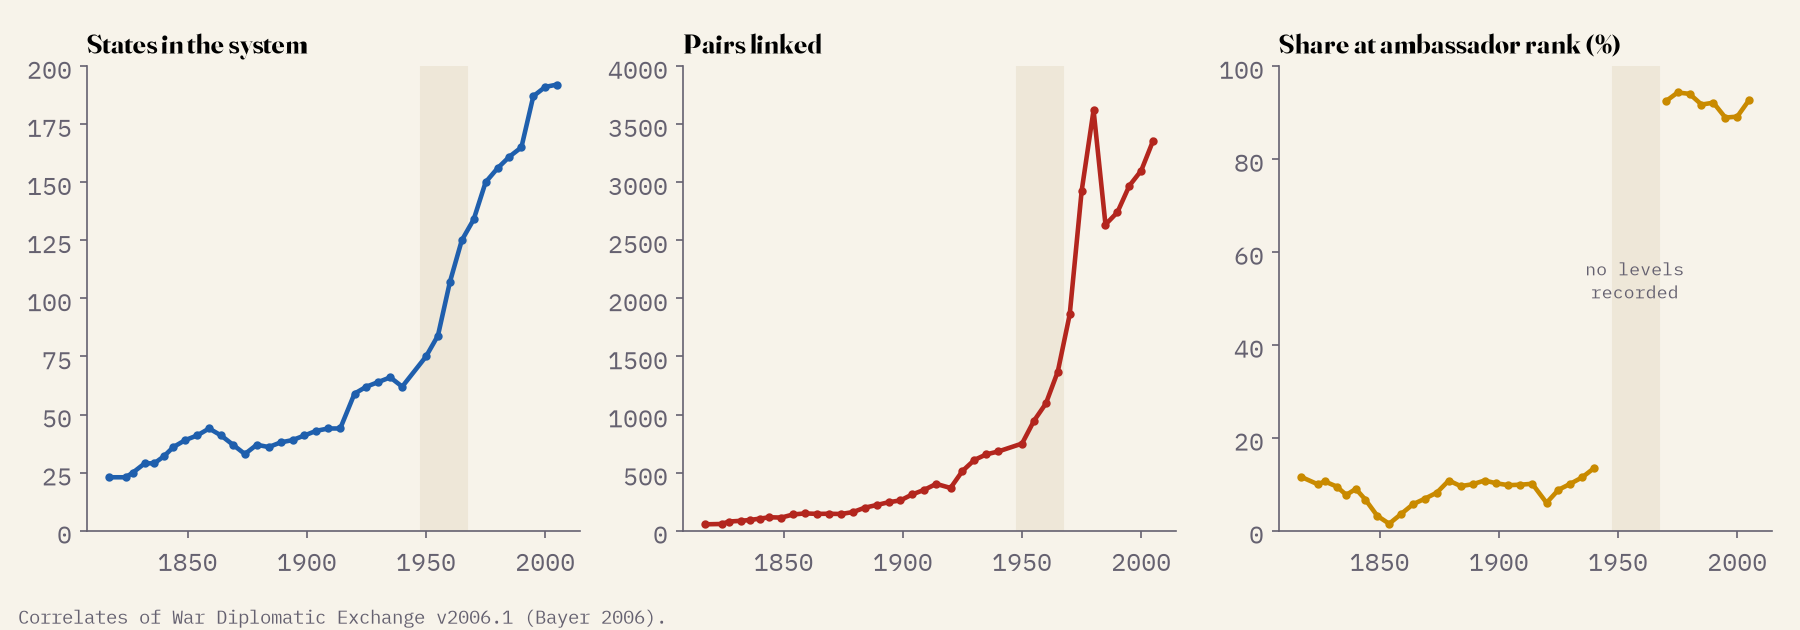
\includegraphics[width=\textwidth]{f_web.png}
\caption{The diplomatic system 1817 to 2005: states, pairs linked and the share of links at ambassador rank (levels not recorded 1950 to 1965, shaded).}\label{fig:web}\end{figure}

\begin{figure}[tbp]\centering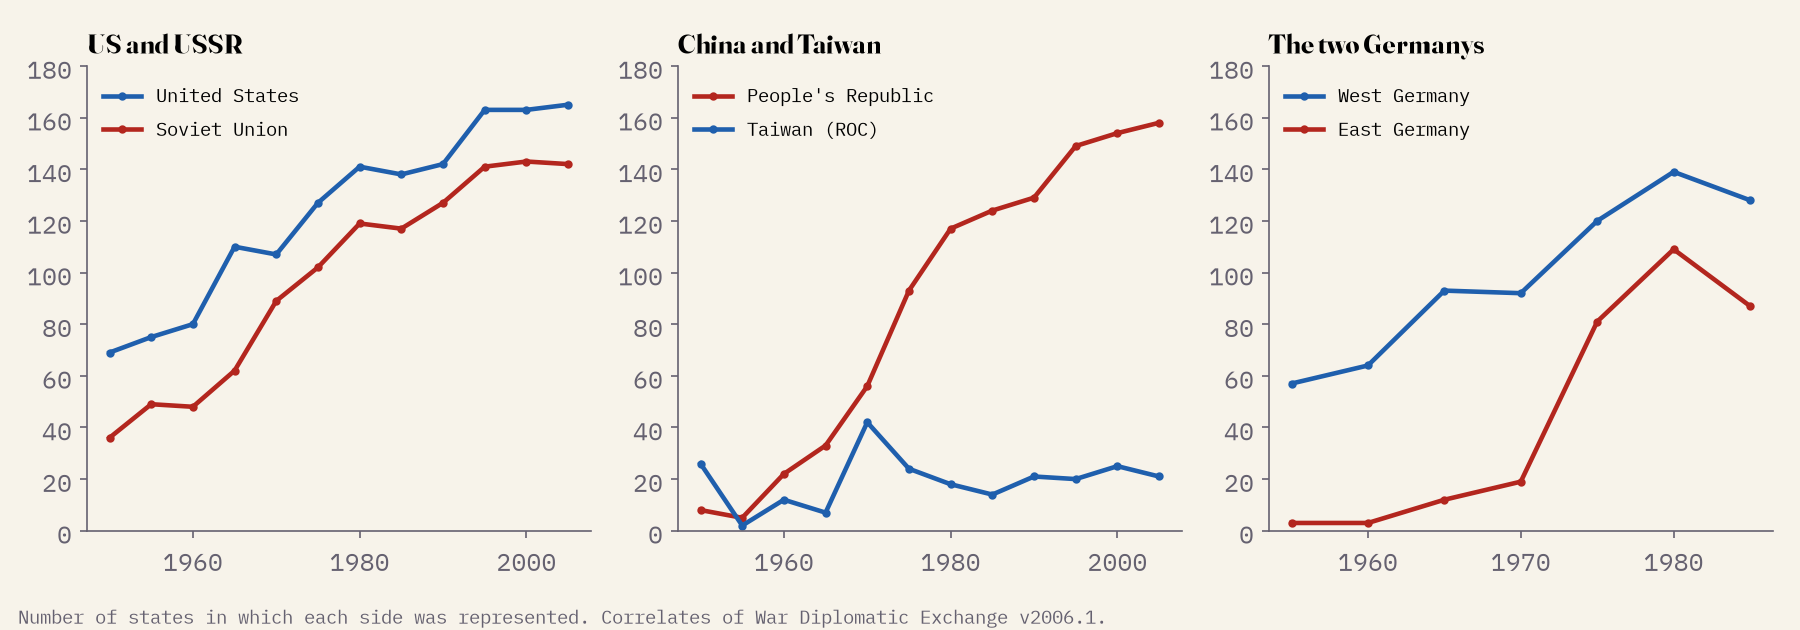
\includegraphics[width=\textwidth]{f_rivals.png}
\caption{Rival networks: number of states in which each side was represented.}\label{fig:rivals}\end{figure}

\subsection{Before 1817}
The deep-history sample (Figure~\ref{fig:deep}, Table~\ref{tab:deep}) runs from 2400 BC to 1815: 8 lines for the Amarna letters, envoys across Eurasia, tribute missions to the Ming, the first resident embassies of Italy from 1446, Spain's resident ambassador in London by 1487 and the first permanent Ottoman embassy in 1793. It is a sample of famous, well-documented cases chosen to illustrate, not a census, and says nothing about the volume of diplomacy in any period.

\begin{figure}[tbp]\centering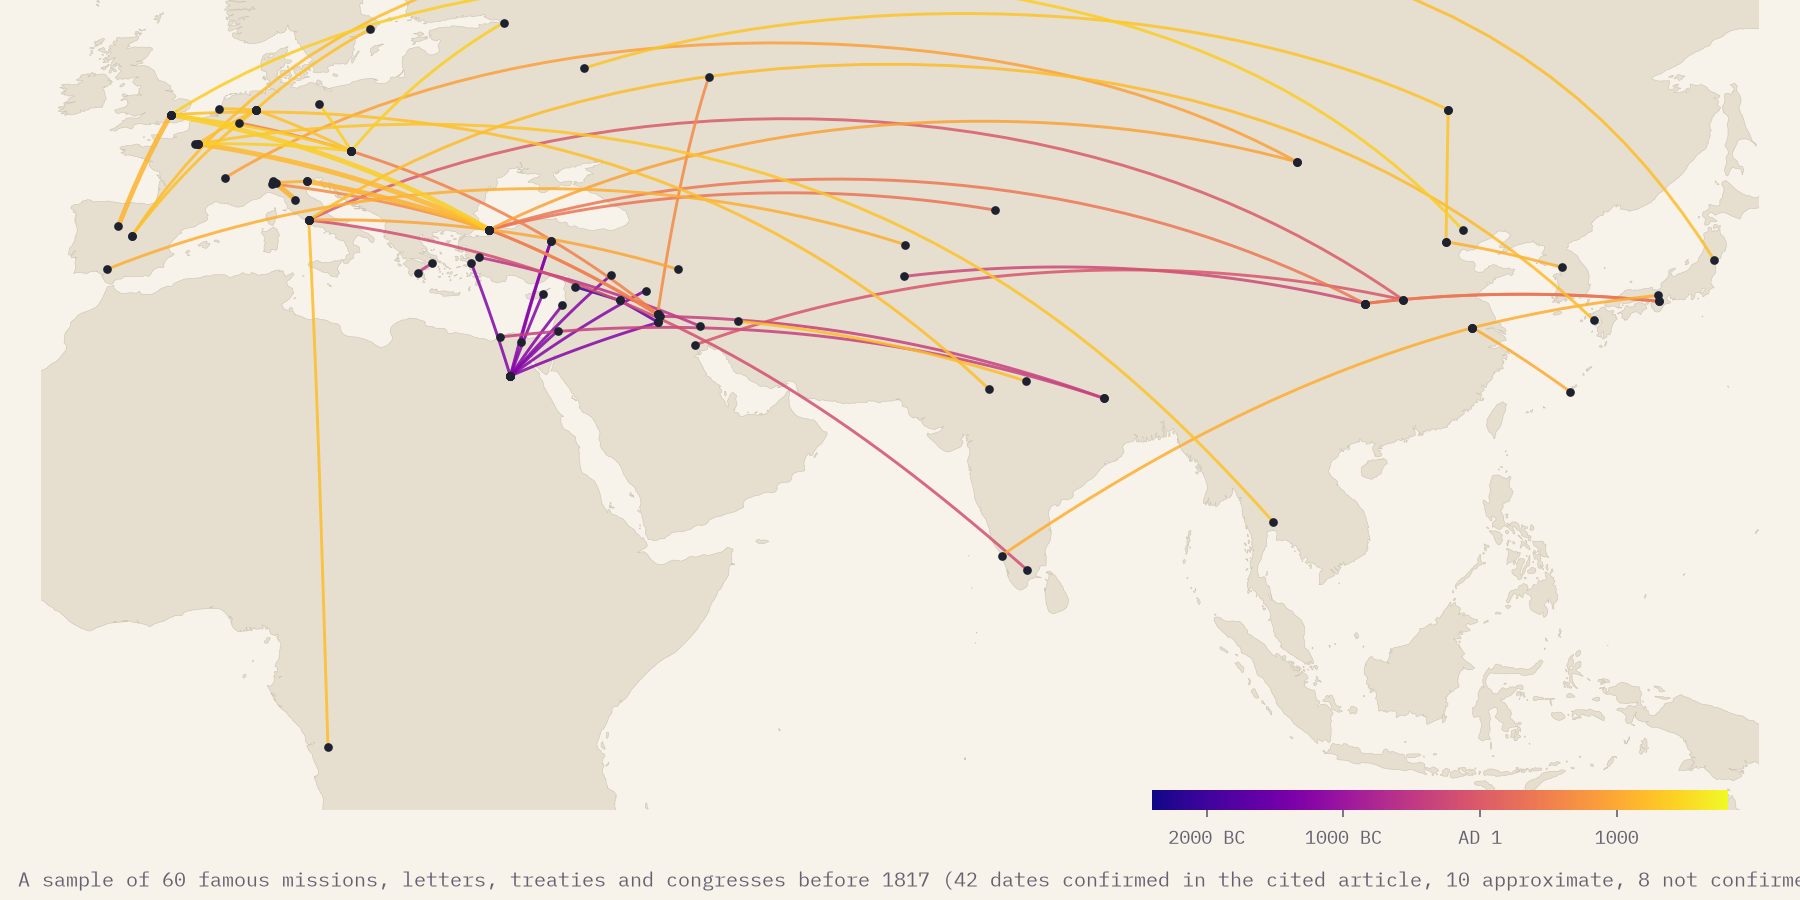
\includegraphics[width=\textwidth]{f_deep.png}
\caption{The deep-history sample, coloured by date.}\label{fig:deep}\end{figure}

{\small\begin{longtable}{p{1.6cm}p{4.5cm}p{3.7cm}p{3.6cm}c}\caption{The deep-history sample: one row per event (congresses and letter networks draw several lines). Sources are English Wikipedia articles. Status: C confirmed (year in the article), A approximate (nearby year), N not confirmed.}\label{tab:deep}\\\toprule Year & Event & Between & Source article & Status\\\midrule\endfirsthead\toprule Year & Event & Between & Source article & Status\\\midrule\endhead
c. 2400 BC & Ebla and Mari & Ebla to Mari & Ebla & C\\
c. 1770 BC & Zimri-Lim and Hammurabi & Mari to Babylon & Mari, Syria & A\\
c. 1350 BC & Amarna letters: Babylon & Amarna (Egypt) to Babylon & Amarna letters & A\\
c. 1350 BC & Amarna letters: Mitanni & Amarna (Egypt) to Washukanni (Mitanni) & Amarna letters & A\\
c. 1350 BC & Amarna letters: Hatti & Amarna (Egypt) to Hattusa (Hatti) & Amarna letters & A\\
c. 1350 BC & Amarna letters: Assyria & Amarna (Egypt) to Assur (Assyria) & Amarna letters & A\\
c. 1350 BC & Amarna letters: Alashiya & Amarna (Egypt) to Alashiya (Cyprus) & Amarna letters & A\\
c. 1350 BC & Amarna letters: Arzawa & Amarna (Egypt) to Apasa (Arzawa) & Amarna letters & A\\
c. 1350 BC & Amarna letters: Byblos & Amarna (Egypt) to Byblos & Amarna letters & A\\
c. 1350 BC & Amarna letters: Jerusalem & Amarna (Egypt) to Jerusalem & Amarna letters & A\\
1259 BC & Egyptian-Hittite peace treaty & Pi-Ramesses (Egypt) to Hattusa (Hatti) & Egyptian-Hittite peace treaty & C\\
c. 500 BC & The Persian Royal Road & Susa to Sardis & Royal Road & N\\
c. 450 BC & Greek proxenia & Athens to Sparta & Proxenos & N\\
c. 302 BC & Megasthenes in India & Seleucia to Pataliputra & Megasthenes & A\\
c. 260 BC & Ashoka's envoys & Pataliputra to Alexandria & Ashoka & C\\
138 BC & Zhang Qian & Chang'an to Bactria (Yuezhi) & Zhang Qian & C\\
c. 20 BC & Indian embassy to Augustus & Madurai (Pandya) to Rome & Indo-Roman trade relations & N\\
AD 97 & Gan Ying & Luoyang to Characene (Persian Gulf) & Gan Ying & C\\
AD 166 & Roman embassy to the Han & Rome to Luoyang & Sino-Roman relations & C\\
AD 562 & Fifty-Year Peace & Constantinople to Ctesiphon & Fifty-Year Peace Treaty & C\\
AD 568 & Maniakh and Zemarchus & Suyab (Western Turks) to Constantinople & Zemarchus & C\\
AD 607 & Ono no Imoko to Sui China & Asuka (Japan) to Chang'an & Ono no Imoko & C\\
AD 630 & First Japanese mission to Tang & Asuka (Japan) to Chang'an & Japanese missions to Tang China & N\\
AD 643 & Fu-lin embassy to the Tang & Constantinople to Chang'an & Sino-Roman relations & C\\
AD 797 & Charlemagne and Harun al-Rashid & Aachen to Baghdad & Abbasid-Carolingian alliance & C\\
c. AD 830 & John the Grammarian & Constantinople to Baghdad & John VII of Constantinople & C\\
AD 921 & Ibn Fadlan & Baghdad to Bolghar (Volga Bulgaria) & Ahmad ibn Fadlan & C\\
AD 949 & Liutprand of Cremona & Pavia to Constantinople & Liutprand of Cremona & C\\
1245 & Giovanni da Pian del Carpine & Lyon to Karakorum & Giovanni da Pian del Carpine & C\\
1253 & William of Rubruck & Constantinople to Karakorum & William of Rubruck & C\\
1287 & Rabban Bar Sauma & Maragheh (Ilkhanate) to Rome & Rabban Bar Sauma & C\\
1372 & Ryukyu tribute to the Ming & Shuri (Ryukyu) to Nanjing & Tributary system of China & C\\
1403 & Ruy Gonzalez de Clavijo & Seville to Samarkand & Ruy Gonzalez de Clavijo & C\\
c. 1404 & Ashikaga missions to the Ming & Kyoto to Nanjing & Japan-China relations & N\\
1405 & Zheng He's first voyage & Nanjing to Calicut & Zheng He & C\\
c. 1420 & Joseon embassies to the Ming & Hanseong (Joseon) to Beijing & Joseon missions to Imperial China & N\\
c. 1446 & The first resident ambassadors & Milan to Florence & Diplomatic mission & N\\
1454 & Peace of Lodi & Venice to Lodi & Peace of Lodi & C\\
c. 1454 & Venetian bailo in Ottoman Constantinople & Venice to Constantinople & Bailo of Constantinople & C\\
c. 1487 & Spain's resident ambassador in London & Medina del Campo (Castile) to London & Rodrigo González de la Puebla & C\\
1535 & France's embassy to the Ottomans & Paris to Constantinople & Franco-Ottoman alliance & C\\
1582 & The Tensho embassy & Nagasaki to Rome & Tensho embassy & C\\
c. 1608 & Kongo embassy to the pope & Mbanza Kongo to Rome & Antonio Emanuele Funta & N\\
c. 1611 & Mughal and Safavid embassies & Agra (Mughal) to Isfahan (Safavid) & Jahangir & C\\
1613 & Hasekura's Keicho embassy & Sendai to Madrid & Hasekura Tsunenaga & C\\
1615 & Sir Thomas Roe & London to Ajmer (Mughal court) & Thomas Roe & C\\
1648 & Peace of Westphalia & Madrid, Munster, Paris, Stockholm, The Hague, Vienna & Peace of Westphalia & C\\
1686 & Siamese embassy to Louis XIV & Ayutthaya to Versailles & Siamese embassy to France (1686) & C\\
1689 & Treaty of Nerchinsk & Beijing, Moscow, Nerchinsk & Treaty of Nerchinsk & C\\
1793 & The Macartney embassy & London to Chengde & Macartney Embassy & C\\
1793 & First permanent Ottoman embassy & Constantinople to London & Embassy of Turkey, London & C\\
1815 & Congress of Vienna & Berlin, London, Paris, St Petersburg, Vienna & Congress of Vienna & C\\
\bottomrule\end{longtable}}

\section{Limitations}
A mapped mission may have closed or suspended work; a missing one may simply not be mapped. Coverage is uneven: by the 2005 benchmark the network abroad looks complete for 185 of 190 states and hosted embassies for 180, but consulates and especially honorary consulates are mapped very unevenly, and some cities (New York's consular corps, the consulates of Western Sahara) are clearly under-mapped. Non-resident accreditation is not represented. The Correlates of War benchmark is twenty years old and coded from different sources. Name matching and type rules are heuristic and some records will be misclassified. The deep-history sample is selective, and 8 of its dates could not be confirmed in the cited articles. Nothing here measures the quality of relations, only presence.

\section{Conclusion}
Open data can now map the world's diplomatic missions with enough completeness to reproduce independent totals for the largest networks. The map shows a dense core of capitals hosting well over a hundred embassies, small states with surprisingly wide networks, capitals that embassies never followed, and a long history in which the resident embassy is a recent invention.

\section*{Data and code availability}
The interactive version is at \url{https://maps.tristanhotham.com/embassies/}. Data and code are at \url{https://github.com/Tristan-Hotham/embassies} and archived with this paper at https://doi.org/10.5281/zenodo.23899269. The mission gazetteer is derived from OpenStreetMap and released under the Open Database License; other derived data are CC BY 4.0 and code MIT.

\section*{AI statement}
I wrote the text, with drafting and editing assistance from Claude (Anthropic), which also helped prepare the analysis code. I reviewed and checked all text and results.

\begin{thebibliography}{9}
\bibitem[Bayer(2006)]{bayer} Bayer, R. (2006) Diplomatic Exchange Data set, v2006.1. Correlates of War Project. \url{http://correlatesofwar.org}
\bibitem[Lowy Institute(2024)]{lowy} Lowy Institute (2024) Global Diplomacy Index 2024: key findings. \url{https://globaldiplomacyindex.lowyinstitute.org/key_findings}
\bibitem[Natural Earth(2026)]{naturalearth} Natural Earth (2026) Admin 0 countries and populated places, 1:10m and 1:50m. Public domain. \url{https://www.naturalearthdata.com/}
\bibitem[OpenStreetMap(2026)]{osm} OpenStreetMap contributors (2026) Diplomatic objects (office=diplomatic, amenity=embassy), via the Overpass API. ODbL 1.0. \url{https://www.openstreetmap.org/copyright}
\bibitem[Reuters(2026)]{reuters} Reuters (2026) Factbox: Taiwan's 12 remaining diplomatic allies.
\bibitem[Wikidata(2026)]{wikidata} Wikidata contributors (2026) Items for embassies, consulates and representative offices. CC0. \url{https://www.wikidata.org/}
\bibitem[Wikipedia(2026)]{wiki} Wikipedia contributors (2026) Articles cited per entry in the deep-history sample (data/deep\_history.csv). CC BY-SA 4.0. \url{https://en.wikipedia.org/}
\end{thebibliography}
\end{document}
